\documentclass{bioinfo}
\usepackage{setspace}

\copyrightyear{2005}
\pubyear{2005}
\usepackage{url}
\usepackage[normalem]{ulem}
\usepackage{multirow}
\usepackage{pifont}
% Load packages
\usepackage{cite} % Make references as [1-4], not [1,2,3,4]
\usepackage{url}  % Formatting web addresses  
\usepackage{ifthen}  % Conditional 
\usepackage[utf8]{inputenc} %unicode support
\urlstyle{rm}
\usepackage{natbib}
\renewcommand{\cite}{\citep}
\usepackage{amsmath}
\usepackage{amssymb}
 
\usepackage{pifont}
%\newcommand{\tick}{\ding{52}}
\newcommand{\tick}{\checkmark}
\newcommand{\tickNo}{\hspace{1pt}\ding{55}}

\begin{document}
\firstpage{1}

\title{Process-based phenotypes: an application to the ontology of
  cell physiology}

\author[Hoehndorf et al.]{Robert Hoehndorf$^1$ and Midori
  A. Harris$^2$ and Heinrich Herre$^3$ and Gabriella Rustici$^4$ and
  Georgios V. Gkoutos$^{1}$}

\address{$^{1}$Department of Genetics, University of Cambridge,
  Downing Street, Cambridge, Cambridge CB2 3EH, UK\\
  $^{2}$Department of Biochemistry; University of Cambridge, 80 Tennis
  Court Road, Cambridge CB2 1GA, UK\\
  $^{3}$Institute for Medical Informatics, Statistics and
  Epidemiology, University of Leipzig, Haertelstrasse 16-18, 04107
  Leipzig, Germany\\
  $^{4}$EBI, Wellcome Trust Genome Campus, Hinxton, Cambridge,
  Cambridge CB10 1SD, UK
}

\maketitle
 
\begin{abstract}
  Phenotypes important for...

  Include behavioral phenotypes, based on behavior ontology

  We identify a problem in representing phenotypes such as drinking
  behavior that...

  provide solution...
\end{abstract}

{\bf Keywords:} cell phenotype, process, ontology, Semantic Web

\section{Introduction}
Phenotype studies on all scales and levels of granularity are now an
invaluable tool for functional genomics research. Phenotypes of
targeted mutations in animal models are now systematically recorded to
reveal the role of individual genes within a biological system. These
phenotype studies now play a key role in translational research and
are being used to reveal candidate genes for orphan diseases and to
identify chemicals that may have effects on these diseases
\cite{Schofield2011}.

The large volume and diversity of phenotypes within different species
and across multiple scales and levels of granularity necessitates the
application of flexible strategies for managing and integrating data
so that it becomes amenable to automated comparative analyses. To
integrate biomedical data across heterogeneous information systems,
biomedical ontologies were being developed \cite{Smith2007}. An
ontology is an explicit specification of a conceptualization of a
domain and can be used to make the meaning of terms in a vocabulary
explicit \cite{Gruber1995, Guarino1998}. They play a crucial role in
the annotation of biomedical data and the integration of model
organism databases \cite{go2010, Bada2004, goble}.

Ontologies increasingly rely on the use of Semantic Web technologies
\cite{Berners-Lee2001}. The Semantic Web provides a stack of protocols
and languages to include explicit semantics in websites. In
particular, the Web Ontology Language (OWL) \cite{Grau2008} has been
designed to express and share ontologies within the Semantic Web. OWL
is a language based on description logics (a group of formal languages
based on first-order predicate logic). Automated reasoners have been
developed within the Semantic Web to perform complex operations on
ontologies formulated in OWL. In particular, automated reasoners can
verify an ontology's consistency and use deductive inference to
perform powerful queries over ontologies. To benefit from automated
reasoning and the rapidly increasing number of software tools that are
being developed within the Semantic Web, most biomedical ontologies
are now available in OWL or can be converted into an OWL-based
representation \cite{Horrocks2007, Hoehndorf2010patterns}.

In the domain of phenotypes, multiple ontologies have been
developed. In particular, ontologies to characterize mammalian
\cite{Smith2004}, human \cite{Robinson2008}, yeast \cite{ypo} and worm
\cite{wpo} phenotypes are now available, while several more phenotype
ontologies are under development. To benefit from automated reasoning,
integrate phenotypes across species and reuse the content of anatomy
and process ontologies, classes in phenotype ontologies were defined
using the framework of the Phenotypic Attribute and Trait (PATO)
ontology \cite{Gkoutos2005}. According to the PATO framework, a
phenotype can be decomposed, using an Entity-Quality model, into an
affected entity and a quality that characterizes {\em how} the entity
is affected \cite{Gkoutos2005}. Such decompositions have been created
for several widely used phenotype ontologies \cite{Mungall2010,
  Gkoutos2009b, obml2011h1}, and are being applied together with
methods for reusing knowledge contained in anatomy ontologies
\cite{Mungall2010, Hoehndorf2010phene}.

While the PATO framework is now successfully being applied to
semantically integrate phenotypes across species, the diversity and
complexity of phenotypes in which biological processes and functions
are impaired continues to limit the interoperability between phenotype
ontologies. Major challenges for representing and integrating
process-based phenotypes include establishing the link to the
components of biological systems that have the capabilities to exhibit
such a behaviour, and that attributes of processes are often measured
{\em indirectly} and inferred from other attributes.

To illustrate these challenges, consider physiological processes of
the heart. One of the heart's functions is {\em Heart beating}, i.e.,
a capability that is realized through processes of the type {\em Heart
  beating}. {\em Blood} is a participant of {\em Heart beating}
processes.  An abnormal phenotype of an organism could be that the
{\em rate of heart beating} is increased. The intended meaning of such
a description is that the number of {\em Heart beating} processes in a
given time interval is higher than normal. Another important attribute
of heart physiology is the fluid flow rate through the heart. For an
abnormal phenotype such as {\em increased rate of fluid flow through
  the heart}, the intended meaning could either be that the amount of
fluid that is moved through the heart within a single heart beating
process is increased or that the amount of fluid that is moved through
the heart within a period of time interval is increased. 

Based on these examples, we can make several observations about
process attributes. First, for a process like {\em Heart beating}, we
can distinguish between single occurrences and processes in which {\em
  Heart beating} occurs multiple times. Only the latter kind of
process may have a {\em rate of heart beating}, while {\em Heart
  beating} processes do not have such an attribute. Second, we can
distinguish between abnormal fluid flow rates in {\em Heart beating}
processes and rate of fluid flow through the heart within a given
duration. Both may have entirely different underlying causes and it is
therefore important to distinguish between them. Finally, we may be
able to infer some phenotypes from others, thereby limiting the number
of phenotypes that must be experimentally observed. For example, when
the fluid flow rate in single heart beating processes is increased and
the {\em rate of heart beating} is increased within a process $P$,
then the rate of fluid flow through the heart will be increased for
$P$.

Here, we present the foundations for an ontology of process
phenotypes. We present the outline of a theory in which several kinds
of process attributes can be distinguished so that normal and abnormal
physiology of biological systems can be formally characterized. We
apply this theory to cellular processes and create the Cell Phenotype
Ontology (CPO). The CPO is linked to reference ontologies for
qualities, biological processes, functions and cell components, and
its prime application is the unification of phenotypes on the cellular
level across different species as well as for annotation of cellular
phenotypes in domains in which no such ontology exists...

\section{Materials and Methods}
\subsection{Formal ontology}
The ontology as an approach to semantic standardisation was proposed
more than a decade ago and since then has become the dominant
methodology used to semantically categorise phenodeviance.  The
biomedical research community has invested considerable amount of
effort and resources in the development and establishment of
ontologies that are becoming increasingly successful as information
management and integration tools in many disparate scientific fields
allowing interoperability and semantic information processing between
diverse biomedical resources and domains.

In computer science, an ontology is a specification of a
conceptualization of a domain of knowledge \cite{Gruber1995,
  Guarino1998}.  Ontologies commonly distinguish between {\em classes}
(also called {\em concepts}, {\em categories} or {\em universals}) and
{\em individuals} within a domain of knowledge. A class is an entity
that can have {\em instances}, while individuals are entities that
cannot be instantiated \cite{Herre2006}. Examples of individuals
include the Eiffel tower or the 2009 Ironman Triathlon in Hawaii,
while examples of classes include {\em Tower} or {\em Triathlon}. The
Eiffel tower can be an instance of the class {\em Tower}, and the 2009
Ironman Triathlon an instance of {\em Triathlon}.  The meaning of
classes is specified by stating what must be true of their instances.

In addition to classes and individuals, ontologies often include {\em
  relations}. Relations hold between entities, they are the ``the glue
that holds things together, the primary constituents of the facts that
go to make up reality'' \cite{Barwise1989}.

In {\em formal} ontologies, the specification of classes and relations
follows the axiomatic-deductive method. Given a set of terms that are
used within a domain and whose meaning we wish to specify, we begin by
providing {\em explicit definitions} for some terms, potentially
introducing new terms. An explicit definition of a term $t$ is a
statement that can replace every occurrence of $t$ in any sentence.

Eventually, a set of {\em primitive terms} remains that are not
further defined. Following the axiomatic method \cite{Hilbert1918},
using only the primitive terms, we can construct complex
sentences. Based on the intended meaning of the primitive terms, we
consider some of these sentences true and some of them false in our
domain. We select some of the true sentences as {\em axioms} which
provide the core of our ontology. Ideally, the axioms are chosen so
that all true sentences in the domain we intend to represent follow by
means of logical deduction from the axioms. More commonly, however,
only {\em some aspects} of the intended meaning are formally
represented while other aspects are omitted either due to limitations
in language expressivity or due to their irrelevance to the problem
for which an ontology is developed.

Based on the axioms and definitions, we can use deduction to infer
statements that logically follow from the axioms.  The process of
automatically deducing sentences from axioms is called {\em automated
  reasoning}. Automated reasoning allows users of an ontology to carry
our key activities: verifying the ontology's consistency, inferring
hidden knowledge and thereby performing powerful queries.  An ontology
is formally inconsistent if there is a statement $\phi$ such that
$\phi$ and its negation $\neg \phi$ can be inferred from the
ontology's axioms.  If an ontology is formally inconsistent, {\em
  every} statement can be inferred from the ontology.  



We assume that the classes of an ontology are
satisfiable, i.e. that they have instances

Classes in an ontology may be unsatisfiable: a class $C$ is
unsatisfiable, if it is not possible that the class has
instances. Unsatisfiable classes are commonly the result of a
contradictory class definition. That a class is unsatisfiable is often
a special kind of unintended consequence that can be drawn from an
ontology.

Automated reasoning in the Web Ontology Language (OWL) can be employed
to automatically compute the generalization hierarchy underlying an
ontology as well as for verification of data consistency and complex
queries \cite{Hoehndorf2011incon, Hoehndorf2011models}. Highly
efficient automated reasoners are available to process OWL ontologies
\cite{Sirin2004, Tsarkov2006, Motik2009a}. OWL profiles were developed
to support even large ontologies by further reducing the expressivity
of OWL in order to enable polynomial-time inferences. In particular
the OWL EL profile was found to provide the expressivity required for
most biomedical ontologies \cite{el4, elvira}, and highly optimized
OWL EL reasoners are available or under development to support
reasoning over very large ontologies \cite{el4, cbreasoner}.

A high expressivity is required to accurately specify complex axioms
that constrain the domain under investigation, and languages with
higher expressivity than OWL are often required in the biomedical
domain to achieve this goal \cite{Hoehndorf2009sequences, rnao}. On
the other hand, automated reasoning over large ontologies and
associated datasets benefits from languages with a low complexity of
inferences in which complex axioms cannot be formulated. Therefore, a
possible solution is to use a layered approach: to specify the meaning
of terms using an expressive language, and derive the axioms that
must obtain in a weaker language using deductive inferences.

\subsection{Processes and their participants}
\begin{figure}
  \centering
  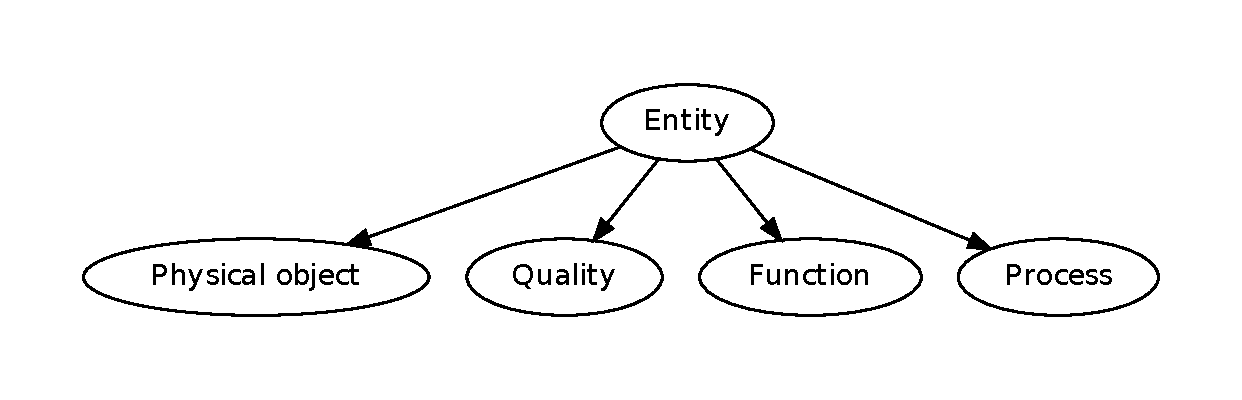
\includegraphics[width=.45\textwidth]{onto.pdf}
  \caption{Overview over basic top-level categories. Physical objects
    are entities that are wholly present at time points. Qualities are
    attributes of entities. Functions are capabilities that arise from
    physical objects with their qualities, and processes are
    temporally extended entities that may be realizations of a
    function.\label{fig:onto}}
\end{figure}

Most biomedical ontologies share common distinctions between different
kinds of entities: physical objects, qualities, functions and
processes. A physical object is an entity that is present as a whole
at a time point, i.e., an entity that has no temporal parts. A quality
is an attribute or feature of an entity. Physical objects together
with their qualities give rise to functions, which are capabilities or
potentials of physical objects. These functions can then be realized
by processes, which are temporally extended entities
\cite{Burek2006}. Examples of classes that may have processes as
instances include {\em Drinking}, {\em Triathlon} or {\em Apoptosis}.
Figure \ref{fig:onto} illustrates these basic categories of being.

Processes commonly have participants\footnote{It may be argued that
  processes necessarily have participants or that processes may have
  no participants. However, these discussions do not affect our aims
  here and take no position in this regard.}. Participants of
processes are entities that are present at time points (i.e., they
have no temporal parts) and may undergo changes during the process
\cite{Herre2006, Herre2010}.  We can further distinguish different
{\em roles} of participation in a process \cite{Loebe2007}. For
example, a runner may participate in a {\em Triathlon} process as a
{\em Runner (role)}, while another person can participate in the same
process but in a different role (such as {\em Referee}).

Amongst the participants of some processes, we will distinguish
between {\em inputs} and {\em outputs} of processes. Chemical
reactions, for example, are processes with definite inputs (the {\em
  reactants}) and outputs ({\em the products}).

\subsection{Gene Ontology}
The Gene Ontology provides a set of ontologies for molecular and
cellular biology, originally designed to support structured
annotations for genes and gene products in all species with respect to
molecular function (MF), biological process (BP) and cellular
component (CC). MF and BP both describe processes, but at different
spatiotemporal scales; in particular, BP includes processes that
unfold within cells and within tissues and organs of multicellular
organisms. Gene product annotations identify participants in the
processes.

Over time, GO development has increasingly emphasized a normalized
approach that includes supplementing existing human-readable text
description with formally specified explicit definitions for GO
classes. The formalization of GO is readily apparent in its
representation of biological regulation.

Regulatory processes may regulate other processes, at either the MF or
BP scale, or biological qualities. GO accordingly includes three broad
categories of regulation terms, regulation of molecular function,
regulation of biological process, and regulation of biological
quality. The first two are explicitly defined entirely with respect to
other GO terms, whereas the third comprises classes in which the
regulated qualities are specified by terms from PATO (see below) or
anatomy ontologies.

All GO regulation terms use one of three relations, {\bf regulates},
{\bf negatively\_regulates} and {\bf positively\_regulates}, to link
regulation terms to process or quality terms. The {\bf regulates}
relations are defined in terms of qualities: a regulatory process
causes a change in magnitude to some quality, which in turn has an
effect on the frequency, rate or duration of some other type of
process. Effects that results in increases and decreases use {\bf
  positively\_regulates} and {\bf negatively\_regulates} respectively
\cite{Mungall2010go}. The existing ontology structure would also
support the addition of subclasses to distinguish, for example,
regulation of the rate of a process from regulation of its duration or
time of onset.

\subsection{PATO and the EQ model}
The Phenotype And Trait Ontology (PATO) was envisaged and designed to
provide a platform for allowing the integration of quantitative and
qualitative phenotype related information across different levels of
granularity of domain knowledge granularity and species
\cite{Gkoutos2005}.  PATO forms an ontology of phenotype qualities
that form basic entities that we can perceive and/or measure such as
colors, sizes, rates etc. One of it's classification axis lies on the
basis of the basic type of entity these qualities inhere to and
distinguishes between qualities of physical objects and qualities of
processes.

PATO allows for the description of affected entities by combining
various ontologies that describe the entities that have been affected,
such as the various anatomical ontologies, GO \cite {Ashburner2000b},
the Cell Type Ontology \cite {Bard2005}, SO \cite {Eilbeck2005} etc
with the various qualities it provides for defining how these entities
were affected.  PATO can be used for annotation either directly in a
so called post-composed (post-coordinated) manner or for providing
formal (logical) definitions (equivalence axioms) to ontologies
containing a set of precomposed (pre-coordinated) phenotype terms. For
instance, to describe the decrease in the length of the sexual cycle
of female animals, we can combine the PATO term \textit{decreased
  duration} ({\tt PATO:0000499}) with the Gene Ontology term
\textit{estrous cycle} ({\tt GO:0042698}), whilst if such a term
existed in a pre-composed ontology (for the {\tt MP:0009007} term from
the Mammalian Phenotype) it could be used to provide an equivalence
statement between that class and the above PATO-based description.

\section{Results}
\subsection{Attributes of processes}
We develop a model of process attributes that is applicable for
representations of physiology and related phenotypes. In principle, we
distinguish between three different kinds of process attributes:
the first are process attributes that arise directly from processes
and include {\em duration} and {\em temporal location}; the second are
attributes that arise from processes and their parts and include {\em
  frequency}; and the third are attributes that arise from processes
and qualities of their participants, and include {\em flow rates}.

Attribute that can be directly linked to a process arise from
processes' temporal extension. For example, a duration is an attribute
that characterizes the temporal extent of a process and is similar to
{\em Length}, {\em Area} and {\em Volume} for one-, two- and
three-dimensional physical objects. A {\em Temporal location}
positions the time interval at which the process occurs with respect
to a reference coordinate system.

However, the majority of attributes that characterize processes are
not based on these types of process attributes alone, but rather
relate attributes of process participants with the duration of a
process. In particular, a {\em rate} typically refers to an attribute
of some entity {\em with respect to an attribute of another entity},
and in the context of processes, rates often refer to attributes of a
process participant with respect to the duration of the process. For
example, a {\em mass flow rate} refers to the {\em Mass} of a process
participant with respect to the duration of the process, i.e., how
much matter is moved (from one point to another) through the process.
As a more complex example, a {\em rate of change of position} refers
to the {\em distance} that an object is moved with respect to the
duration of the process.

However, not all rates of a process depend on attributes of the
process participants. In particular, a {\em frequency of occurrence}
or {\em event rate} refers to the number of occurrences of a type of
process during a reference process. For example, a {\em rate of heart
  beating} refers to the number of {\em Heart beating} processes that
occur within a reference process (e.g., a process in which the heart
participates with a duration of one minute). Further attributes that
depend on types of processes with regard to a reference process are
{\em distribution patterns}, i.e., how the occurrences of processes of
a particular type are distributed within a reference process. For
example, the heart may beat {\em rhythmically} or {\em arrhythmically}
within a period of time.

Related to distribution patterns are {\em changing qualities} of
processes. For example, the rate of heart beating may change ({\em
  increase} or {\em decrease}) throughout the course of a reference
process. A simple analysis of {\em increasing} ({\em decreasing})
rates would be that the rate of a heart beating within the first half
of a process is {\em lower} ({\em higher}) than in the second half of
the process. To make such an assertion, we divide a process into two
temporal parts. Mathematically, this process of sub-division can be
iterated until processes occur within infinitesimally small time
intervals.

While some processes can be subdivided indefinitely without changing
the type of process, others cannot. A class $C$ of {\em continuous
  processes} is a class that has processes $p$ as instance such that
all temporal parts of $p$ are also instances of $C$. Examples include
{\em continuous movements} or {\em mass flow} processes. On the other
hand, {\em discrete processes} can be subdivided into stages of
activity and stages of inactivity: a class $C$ of {\em discrete
  processes} is a class with processes $p$ as instance and there is a
part of $p$ that is not an instance of $C$. An example is {\em heart
  beating} which has periods of activity (a single heart beat) and
inactivity.

We may further attribute a {\em frequency} or {\em rate} to an object
instead of a process. For example, a heart that beats {\em now} with a
frequency of 80 beats per minute, or a car that is moving at a speed
of 180 kilometres per hour {\em at a particular point in time} (e.g.,
as observed with a speed camera) can be considered attributes of the
objects (the heart or the car), not attributes of the processes in
which the objects participate. However, these are {\em different}
kinds of attributes. Rates, when considered as attributes of objects,
may be explicitly defined using rates of processes. For example, the
heart beating frequency of a particular heart $h$ at a time point $t$
is the frequency of a reference heart beating process in which $h$
participates. Such a reference process is necessary in order to obtain
a value for a frequency even when no {\em heart beating} process is
occurring. However, the frequency is only an attribute of the heart in
virtue of such a reference process in which {\em heart beating} is
actually occurring.  This reference process can be uniquely determined
for continuous processes (such that the frequency or rate of an object
at a time $t$ is the frequency or rate of the infinitesimally small
process around $t$), and is ambiguous for discrete processes (in which
case the reference process must be explicitly stated).

Figure \ref{fig:patterns} illustrates some examples of
non-comparative and comparative process attributes.

% A similar construction as for continuous processes can be made for
% discrete processes. A rate of blood flow is immediately an attribute
% of a single heart beat process. However, during a period of time, the
% cumulative rate of blood flow can be observed as the sum of the blood
% flow rates of individual heart beating processes.

\begin{figure}
  \centering
  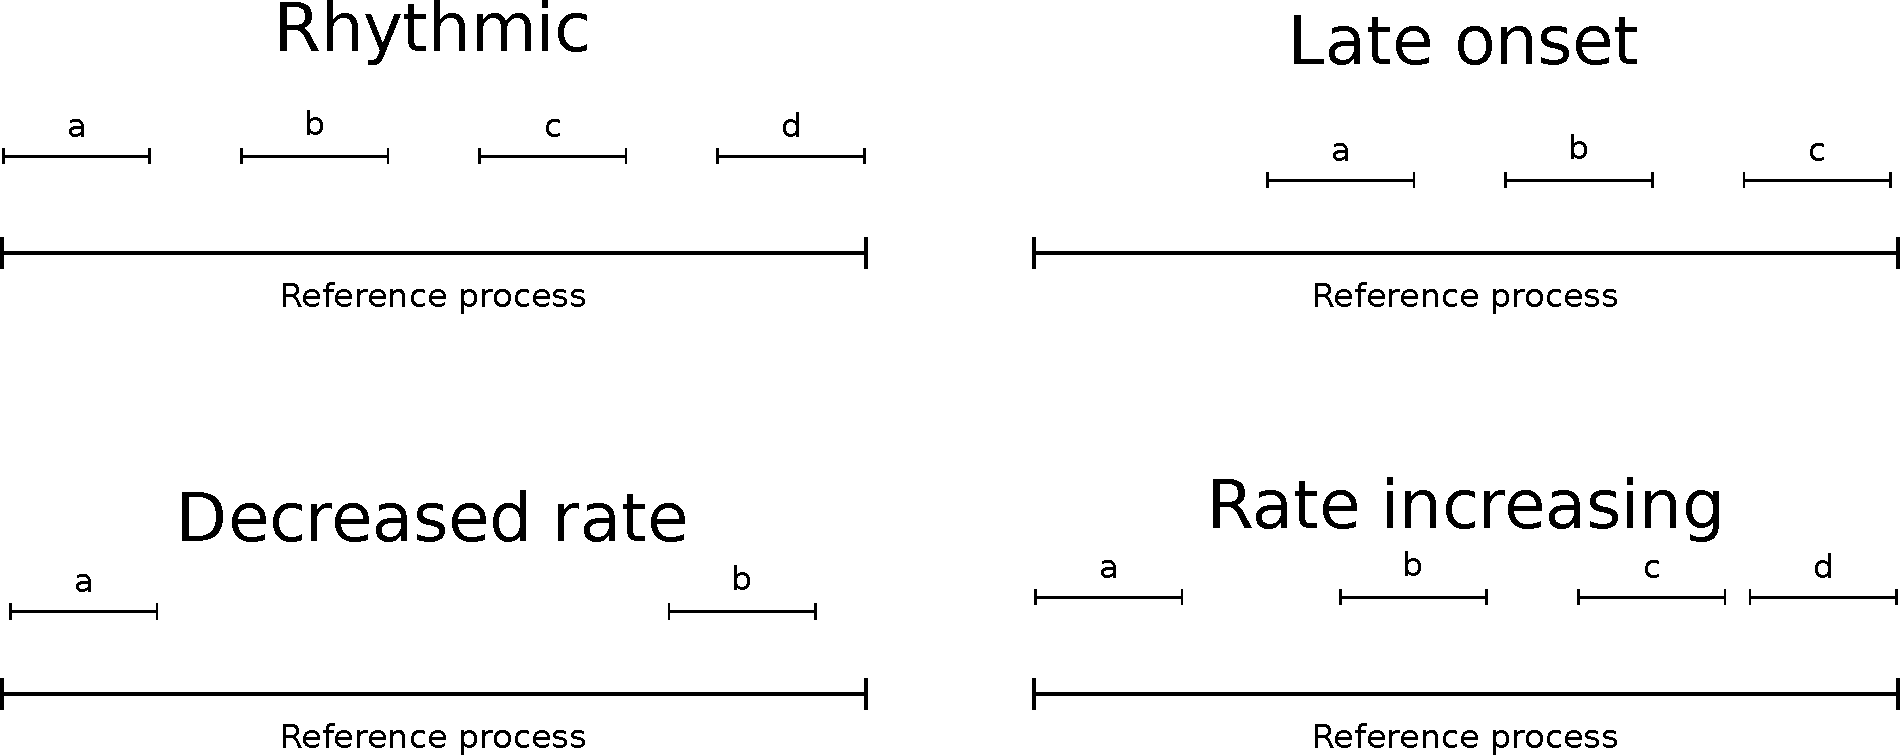
\includegraphics[width=.5\textwidth]{processpatterns.pdf}
  
  \caption{\label{fig:patterns}Six examples of processes with
    non-comparative and comparative process attributes.  We assume
    that the processes labelled $a$, $b$, $c$ and $d$ are all
    instances of the class of processes $P$.  On the left side, three
    regulation (of $P$) processes are illustrated which exhibit
    non-comparative attributes. The first process has an attribute of
    {\em rhythmic} occurrence of $P$ because the instances of $P$ are
    temporally equidistantly distributed. The second example shows an
    {\em arrhythmic} occurrence of $P$, and the third examples shows
    an {\em increasing frequency} (of $P$). A regulation process with
    an increasing frequency (of $P$) is a process in which the
    frequency of occurrences of $P$ is lower in the first half of the
    process than in the second half. The right side of the figure
    illustrates comparative phenotypic descriptions of processes. On
    the upper right, the {\em normal} reference is shown. The second
    example illustrates a {\em late onset} of $P$, i.e., the attribute
    that $P$ processes begin later than {\em normal}. Finally, the
    lower right illustrates a {\em decreased frequency} (of $P$),
    since fewer processes of the type $P$ occur within the reference
    process than {\em normal}.}
\end{figure}

% Complex relations between Based on these definition patterns,
% interdependencies between process attributes can be observed.

\subsection{Cell Phenotype Ontology}
\begin{figure*}[h]
  \centering
  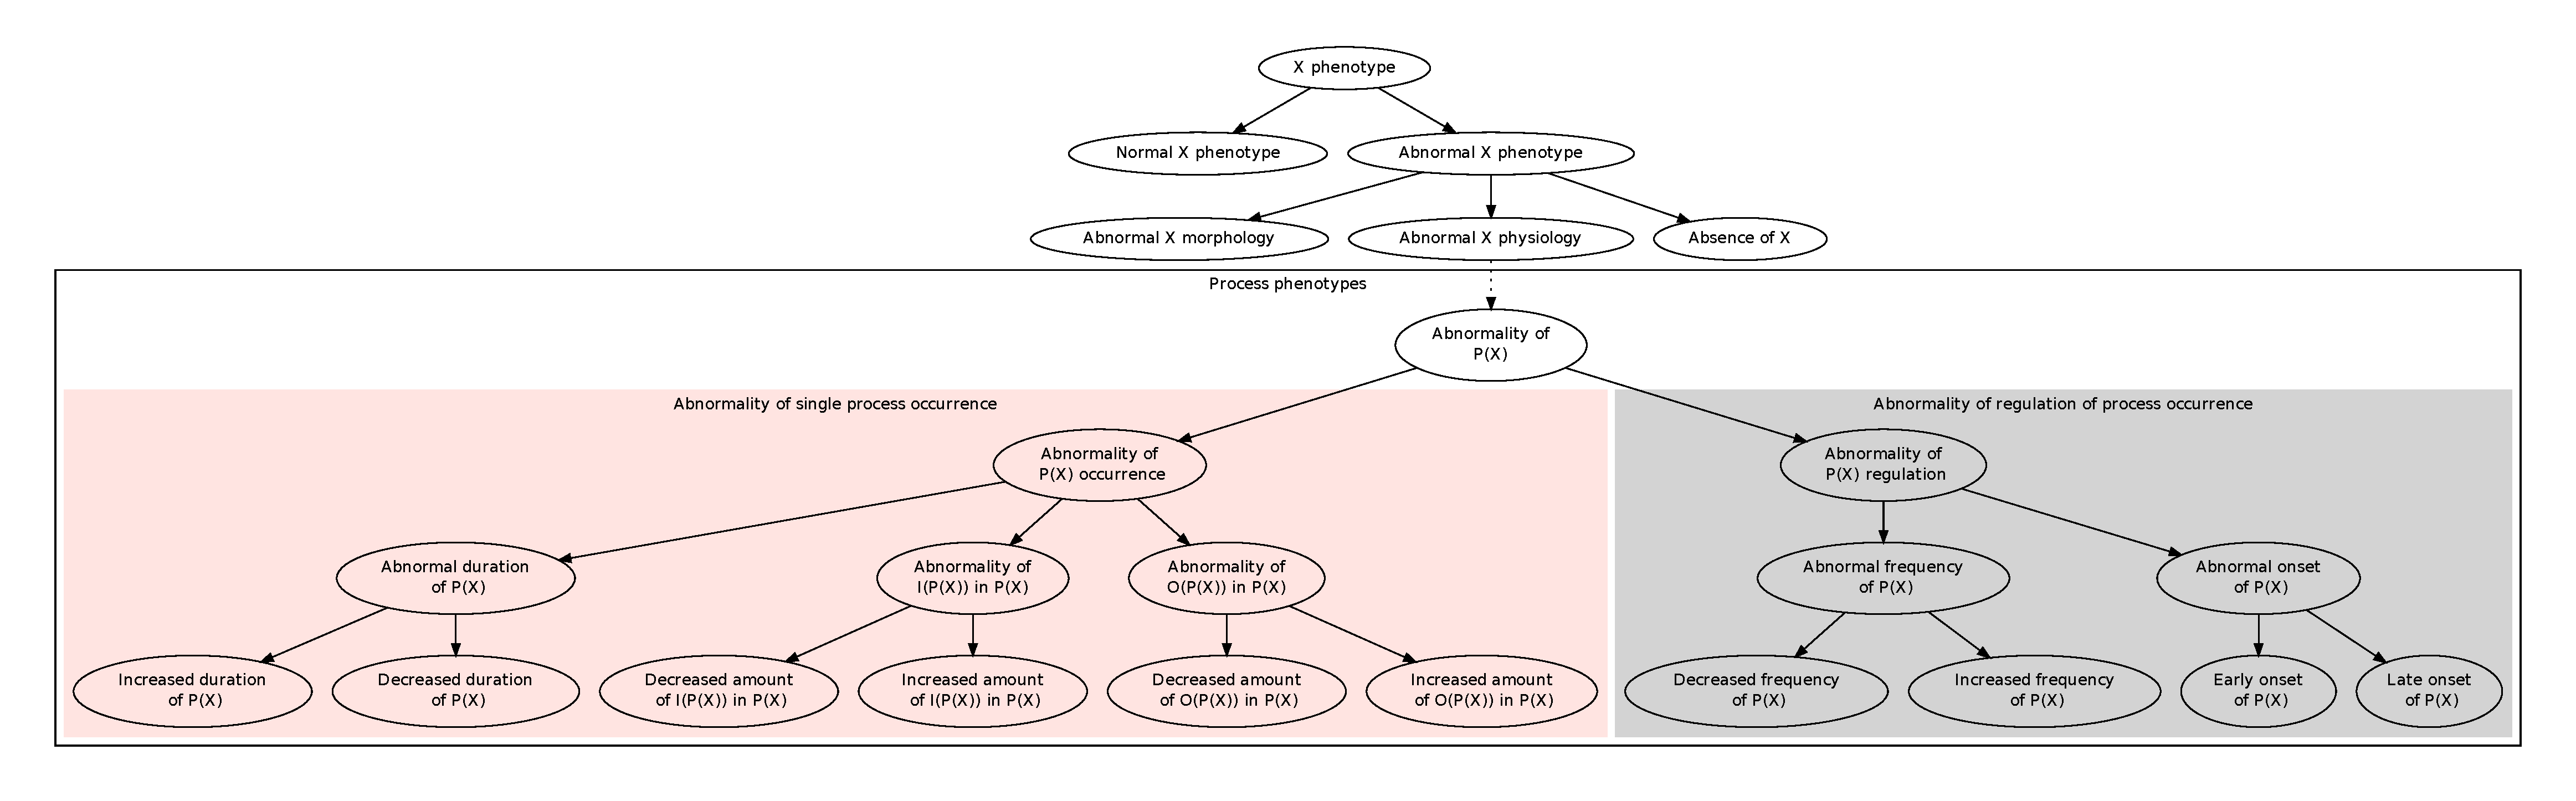
\includegraphics[width=\textwidth,
  height=.33\textheight]{overview.pdf}
  \caption{Overview over ...\label{fig:overview}}
\end{figure*}

While our considerations about process attributes are only the
beginnings of a full-fledged theory, we have derived several phenotype
formalization patterns and a high-level taxonomic structure of
process-based phenotypes. To evaluate our approach, we created the
Cellular Phenotype Ontology (CPO) by automatically applying our
patterns to the GO.

% CPO contains both structural abnormalities and physiological
% abnormalities of cells.
Phenotypes in the CPO are either based on structural abnormalities or
abnormal physiology involving cells or cell components. Structural
abnormalities in the CPO are based on GO's Cellular Component (GO-CC)
hierarchy. GO-CC contains 2,918 classes for cell parts (including {\em
  Cell}) and extracellular components of cells. For each cellular
component class $C$ in the GO-CC, we create a new class labelled {\em
  $C$ phenotype} in the CPO. For example, for the class {\em
  Mitochondrion} ({\tt GO:0005739}) in the GO-CC, we create the class
{\em Mitochondrion phenotype}.

Amongst the structural phenotype classes, we first distinguish between
{\em normal} and {\em abnormal} phenotypes. An {\em Abnormal phenotype
  of $C$} is a phenotype of an organism that does not have a normal
$C$ as part, while a {\em Normal phenotype of $C$} represents the
state in which an organism has a {\em normal $C$} as part.

Amongst the abnormal phenotypes that we include for all cell
components listed in GO-CC, we distinguish {\em abnormal morphology}
and {\em abnormal physiology} phenotypes. An {\em Abnormal morphology
  of $C$} is either the (abnormal) absence of required parts of $C$,
the (abnormal) presence of additional parts, or abnormal qualities of
$C$ \cite{Hoehndorf2010phene}. For example, an absence of caveolae
({\tt MP:...}) would be a subclass of {\em Abnormal morphology of
  plasma membrane} in virtue of caveolae necessarily being part of the
{\em Plasma membrane} ({\tt GO:0005886}).

Abnormal physiology of a cell component refers to abnormal {\em
  functionality} of a cell component. We assume that a functionality
of a cell component is (the potential for) a process in which the cell
component is (causally) involved. We use the definitions of GO classes
that were created based on lexical decompositions of GO class labels
\cite{Mungall2010go, Bada2007a, Ogren2004} to identify the processes
in which cell components are involved. For example, the definition of
the GO class {\em Mitochondrial fission} ({\tt GO:0000266}) is
explicitly defined as an {\em Organelle fission} ({\tt GO:0048285})
that {\bf results-in-the-division-of} a {\em Mitochondrion} ({\tt
  GO:0005739}). Based on this definition, we make the assumption that
{\em Mitochondrial fission} is one of the functions of a {\em
  Mitochondrion} and that an {\em Abnormality of mitochondrial
  fission} is a subclass of an {\em Abnormality of mitochondrion
  physiology}.

Amongst abnormal physiology, we distinguish between abnormalities in a
{\em single occurrence} of a cell component's functioning and an
abnormal {\em pattern of multiple occurrences} of a cell component's
functioning. For example, abnormalities in cell division resulting in
{\em Aneuploidy} refer to abnormalities of functioning processes,
while an {\em increased rate of cell division} refers to an
abnormality in the pattern of occurrence of multiple cell division
processes. In the CPO, abnormalities in the pattern of occurrence of
$X$ are represented as abnormalities in the {\em regulation of $X$}.

Single occurrences of processes can be abnormal in multiple ways,
depending on the type of process.
%
First, common to all processes is the quality of {\em duration} and
consequently, each process can have an {\em abnormal} (increased or
decreased) duration. For example, a part of an organism may
participate in an {\em Inflammatory response} ({\tt GO:0006954}) that
lasts longer than normal, i.e., the organism has an {\em Increased
  duration of inflammatory response} phenotype. We define such a
phenotype as a phenotype of an organism which has a part that
participates in {\em Inflammatory response}, and this {\em
  Inflammatory response} process has an {\em Increased duration} ({\tt
  PATO:0000498}).

The second common type of abnormality are abnormalities based on
process participants in relation to the duration of the process. These
include all kinds of {\em rates} such as {\em mass flow rate}, {\em
  energy flow rate} and {\em velocity} (the rate of change of
position). In each of these cases, an object participates in a process
and a quality (or change of quality) of that object throughout the
duration of the process is considered to form a new quality. If the
process has participants that are distinguished into {\em inputs} and
{\em outputs}, then a recurring pattern is that the amount of inputs
or outputs that participate in the process can be {\em increased} or
{\em decreased}. For example, an {\em Increased rate of cytoplasmic
  streaming} can be defined as an increased amount of inputs or an
increased amount of outputs of a {\em cytoplasmic streaming} process.

Finally, some objects may be divided into stages during which
particular states of affairs obtain, and a process may be abnormal in
that these states of affairs do not obtain at a particular
stage. Notably, at the beginning and the end of a process, pre- and
post-conditions may obtain that are abnormally changed in a
process. For example, {\em Aneuploidy} -- an abnormality during cell
division at which the chromosomes do not separate properly between the
two cells -- may be considered the result of such an abnormality.

We implement the first two types of abnormality in the CPO. First, as
a subclass of each {\em Abnormality of P} class, we create {\em
  Abnormal duration of P}, which in turn has {\em Increased duration
  of P} and {\em Decreased duration of P} as subclasses. Second, if we
are able to identify {\em inputs} $I(P)$ or {\em outputs} $O(P)$ of
the process $P$ in the formal definitions of the GO, we automatically
generate {\em Abnormality of $I(P)$ in $P$} as well as {\em
  Abnormality of $O(P)$ in $P$}.  The left side of Figure
\ref{fig:overview} illustrates the schema of classes we generate for
single process abnormalities.

The second type of abnormality in the CPO relate to abnormalities of
{\em multiple} occurrences of some process $X$. According to the GO,
{\em regulation} processes are processes that maintain or modify the
occurrence of processes of a particular type. Following this
convention, we call an abnormality of multiple occurrences of $X$ {\em
  abnormality of the regulation of $X$}.

A first kind of abnormality of regulatory processes are {\em abnormal
  temporal distribution patterns} of a process. In these
abnormalities, the {\em way} in which processes of a particular kind
are temporally distributed is abnormal.  The most common abnormal
distribution pattern is an increased or decreased frequency, and we
use PATO's {\em frequency} class to define {\em Abnormal frequency of
  occurrence of $X$}.
% \begin{verbatim}
% has-phenotype some (has-part-some (participates-in some 
%   (regulates some X and has-quality some (frequency and towards some X))))
% \end{verbatim}
For example, an {\em Abnormal frequency of occurrence of apoptosis} is
defined as an abnormality of {\em Regulation of apoptosis} ({\tt
  GO:0042981}) with respect to the {\em frequency} ({\tt
  PATO:0000044}) of {\em Apoptosis} ({\tt GO:0006915}) occurrences.

There are further types of deviation from a distribution pattern. For
example, a kind of process that is normally {\em rhythmic} can be
abnormal in that it is {\em arrhythmic}. A typical example of this
kind of process is {\em Heart beating} ({\tt GO:0060047}), in which
{\em Cardiac muscle contraction} ({\tt GO:0060048}) processes occur in
a rhythmic pattern. In {\em Cardiac dysrhythmia}, however, {\em
  Cardiac muscle contraction} processes occur arrhythmically, and we
consider this to be an abnormality of the regulation of {\em Cardiac
  muscle contraction}. While these abnormalities are often highly
informative in clinical diagnostics and biological investigations, we
usually lack the necessary information that is required to
automatically determine meaningful types of abnormal distribution
patterns.

A second kind of regulatory abnormalities is related to the {\em
  onset} of a process. With respect to a reference process, a
particular kind of process may be {\em delayed} ({\tt PATO:0000502})
or {\em premature} ({\tt PATO:0000694}). For example, {\em Delayed
  apoptosis} refers to an abnormality of the {\em Regulation of
  apoptosis} in which apoptosis is induced later than normal.  We use
the PATO quality {\em onset} ({\tt PATO:...}) and its children {\em
  delayed} and {\em premature} to define these types of regulatory
abnormality. Similarly, we use PATO's {\em offset} ({\tt PATO:...})
  quality and its children to characterize regulatory abnormalities in
  which a process ends prematurely or too late.

\begin{table*}
  \centering
  \begin{tabular}{l|l|l|l}
    & Increased cytoplasmic flow rate & Normal cytoplasmic flow rate & Decreased
    cytoplasmic flow rate \\
    \hline
    Increased frequency &increased total flow rate &increased total
    flow rate &?\\
    Normal frequency &increased total flow rate &normal total flow
    rate &decreased total flow rate\\
    Decreased frequency &?&decreased total flow rate &decreased total
    flow rate\\
    \hline
  \end{tabular}
  \caption{\label{tbl:flow}Interdependency for the attribute {\em
      Total cytoplasmic flow rate}. Depending both on whether the
    cytoplasmic flow rate in individual {\em cytoplasmic streaming}
    processes is increased or decreased and whether the frequency of
    occurrence of {\em cytoplasmic streaming} is increased or
    decreased, the total cytoplasmic flow rate can be increased or
    decreased.}
\end{table*}

Finally, a third kind of regulatory abnormality refers to abnormal
rates with respect to a participant of the process that is being
regulated. For example, a cytoplasmic flow rate can be increased or
decreased not within a single {\em cytoplasmic streaming} process but
rather the total cytoplasmic flow rate, as a summation over all
cytoplasmic streaming processes that occur within an organism (or a
particular anatomical location), is increased or decreased. While a
flow rate of a single {\em cytoplasmic streaming} process is a quality
of that process, an increased {\em total} cytoplasmic flow rate is a
quality of the regulation of {\em cytoplasmic streaming}. In
particular, it is possible for an organism to have a normal --- or
even a decreased --- cytoplasmic flow rate in each individual
cytoplasmic streaming process while at the same time having an
increased total cytoplasmic flow rate due to a large increase in the
frequency of occurrence of cytoplasmic streaming processes. Similarly,
the frequency of occurrence of cytoplasmic streaming may be normal or
decreased while the total cytoplasmic flow rate is increased due to an
increased cytoplasmic flow rate in each individual cytoplasmic
streaming process. Table \ref{tbl:flow} illustrates the dependencies
between rates of individual processes, their frequency of occurrence
and the total rate of these processes. We include total rates as
regulatory abnormalities in the CPO since these are the attributes of
processes that are often measured or observed, while the rates of
individual processes are inferred following a schema such as Table
\ref{tbl:flow}.

\subsection{Implementation}
We were faced with two choices for implementing the CPO: we could
either implement a pre-composed ontology in which all classes and
their definitions are pre-generated according to the patterns we
define, or we could develop an annotation software that enables the
selection of our process phenotype patterns based on the current
structure of the GO.  To maximize the utility and compatibility of the
CPO, and to provide stable identifiers for its concepts, we selected
the first strategy and developed a software to automatically generate
a pre-composed ontology from the GO.

We developed a software that utilizes the OWL API \cite{Horridge2007}
in order to generate an OWL representation of the CPO. The software
requires three input files: a version of the GO on which to base the
generated CPO, a version of PATO that is used to define abnormal
qualities, and a copy of the GO cross-product definitions
\cite{Mungall2010go} that is used to relate cell components to the
processes in which they participate as well as identify the
participants, inputs and outputs of processes.

We automatically generate a unique numerical identifier for each class
in the CPO.  Since the CPO is based on the GO and need to be updated
with subsequent versions of the GO, we must ensure to keep identifiers
stable in subsequent versions of CPO. Therefore, we use the
identifiers for GO classes to generate CPO class identifiers.

In the CPO, identifiers contain two components and are of the form
{\tt CPO:XXGGGGGGG}, where {\tt GGGGGGG} is the seven-digit identifier
of the GO class on which the CPO class is based, and {\tt XX} is a
prefix that identifies the type of phenotype pattern that is applied
to the GO class. For example, based on the class {\em Apoptosis} ({\tt
  GO:0006915}), we generate the CPO classes {\em Abnormality of
  Apoptosis}, {\em Abnormality of single occurrence of apoptosis} and
{\em Abnormality of regulation of apoptosis}.  We use the prefixes
{\tt 12}, {\tt 14} and {\tt 15} for each of the corresponding
phenotype patterns, and consequently generate the class identifiers
{\tt CPO:120006915}, {\tt CPO:140006915} and {\tt CPO:150006915}. As
long as the GO maintains its identifier for the {\em Apoptosis} class,
the identifiers in the CPO will remain stable even when it is
regenerated.

We use the labels of GO classes to automatically generate class labels
for phenotype classes as well as textual definitions for classes in
the CPO. For example, the label of the class for increased number of
occurrences of {\em Apoptosis} is {\em Increased frequency of
  occurrences of Apoptosis}, and its textual definition states: ``An
increased frequency of occurrences of Apoptosis is a phenotype of
entities in which the number of occurrences of Apoptosis within a
given time period is increased in comparison to a reference process.''

When using the GO and PATO ontologies from 30 Nov 2011, CPO contains
XX classes...
Classifies in...

\section{Discussion}
\subsection{Use of CPO}
The Fission Yeast Phenotype Ontology (FYPO), a new ontology developed
to support annotation of phenotypes in {\em Schizosaccharomyces
  pombe}, consists of pre-composed terms describing normal or abnormal
cellular phenotypes. Over 80\% of FYPO definitions reference
descendants of GO BP 'cellular process' as the entity; a further 11\%
reference GO CC terms. All FYPO explicit definitions reference
qualities in PATO, including {\em normal}, {\em abnormal}, and several
process qualities including {\em increased duration}, {\em decreased
  occurrence}, etc. FYPO will thus fit neatly under the CPO umbrella,
and stands to benefit from the automated synchronization between CPO
and GO. {\em S. pombe} annotations to FYPO terms will provide a rich
body of highly specific, well-supported data to be integrated with
data from other species.

%%%%%%%%%%%%%%%%%%%%%%%%%%%%%%%%%%%%%%%%%%%%%%%%%%%%%%%%%%%%%%%%%%%
A domain that would greatly benefit from the development of a CPO is
Systems Microscopy, which aims to understand complex and dynamic
cellular systems by combining automated fluorescence microscopy, cell
microarray platforms, quantitative image analysis and data mining
(Lock \& Stromblad, Exp. Cell Res. 2010).

If we consider some of the studies, which have been published in this
field in the last few years (Neumann et al, Nature 464: 722-727;
Schmitz et al, Nature Cell Biology 12: 886-893; Fuchs et al, Mol Sys
Biology 6: 370), the need for a CPO becomes evident.

In all three studies here considered live-cell imaging assays and RNAi
knockdown were used to generate phenotypic profiles that quantify the
cellular response to a given siRNA thus allowing identification of
hundreds of genes involved in diverse biological functions including
cell division, migration and survival.

In each study, several phenotypes were detected and described by the
authors without the use of ontologies (see table), making the
integration between datasets extremely difficult. For example, it is
evident that cell division phenotypes were observed in the three
datasets (e.g. 'Mitotic delay/arrest' and 'Prolonged mitotic exit' or
'Methaphase delay' and 'Methaphase cells') but the overlap between
such phenotypes is unclear.

Data integration is also complicated by the lack of standardization at
the level of data production and processing; all these issues are
currently being address by the different groups involved in the
Systems Microscopy Network of Excellence
(http://www.systemsmicroscopy.eu/) and the first step towards data
integration will be achieved by developing a CPO.

This ontology will be used to integrate phenotypes' definitions across
existing datasets and will then become an integrated part of the data
processing pipeline and used to annotate the data as it gets generated
(Conrad et al, Nature Methods 8: 246-249).

\subsection{Pre- vs. post-composed ontology}
We implemented the CPO using a pattern-based approach to formulating
phenotypes involving processes. The patterns we identify use
pre-existing ontologies, in particular the PATO ontology and the
classification of cellular processes as well as cellular components in
the GO. The result is a large ontology in which classes for phenotypes
are {\em pre-composed}: they are named and defined within an OWL
ontology. However, the large size of the resulting ontology may impair
its utility for data annotation and integration, and software tools
may not always support such very large ontologies. The alternative to
pre-composing all possible phenotype classes using the patterns we
describe is to dynamically generate appropriately defined classes at
the time at which they are being used. To achieve this goal, software
must be developed to support ontology users in applying these patterns
and generate the appropriate class description when required.

% \subsection{Future work}
% Formal, axiomatic system for process qualities, maybe based on PSL,
% FOIS paper 2010

% one example:...

% \subsection{Conclusion}

\section{Acknowledgements}
MAH is supported by Wellcome Trust grant WT090548MA.

% % %%%%%%%%%%%%%%%%%%%%%%%%%%%%%%%%
% \section*{Authors contributions}

    
% % %%%%%%%%%%%%%%%%%%%%%%%%%%%
% The authors declare that they have no competing interests.

% % %%%%%%%%%%%%%%%%%%%%%%%%%%%
% \section*{Acknowledgements}
% \ifthenelse{\boolean{publ}}{\small}{}

% The research work in its first unrevised form was presented at the
% SMBM 2010, Hinxton, Cambridge, U.K.


 
%%%%%%%%%%%%%%%%%%%%%%%%%%%%%%%%%%%%%%%%%%%%%%%%%%%%%%%%%%%%%
%% The Bibliography %%
%%                                                         %%
%% Bmc_article.bst will be used to %%
%% create a .BBL file for submission, which includes %%
%% XML structured for BMC.  %%
%%                                                         %%
%%                                                         %%
%% Note that the displayed Bibliography will not %%
%% necessarily be rendered by Latex exactly as specified %%
%% in the online Instructions for Authors.  %%
%%                                                         %%
%%%%%%%%%%%%%%%%%%%%%%%%%%%%%%%%%%%%%%%%%%%%%%%%%%%%%%%%%%%%%


\bibliographystyle{plain} % Style BST file
\bibliography{lc}

\end{document}
